After having regarded the theoretical foundations of streaming, we now look at existing implementations of stream transport and processing platforms that are available to the public (some companies have custom platforms for internal use only). We will regard them under the aspects of correctness, fault tolerance, latency and scalability.





\section{Stream Transport Platforms}
Stream transport platforms are responsible for moving streams between producers and consumers, but may also store them for replay. Theoretically, any message queue or publish--subscribe message broker like ActiveMQ, Pulsar or RabbitMQ but also hosted services like Google Cloud Pub/Sub\footnote{\url{https://cloud.google.com/pubsub}} could be used for this task. However, these neither provide the end-to-end exactly-once\footnote{RabbitMQ has limited support for being used as exactly-once source but not as exactly-once sink since transactions are not supported~\cite{Apache.2020}. Pulsar can be used as exactly-once source using the same mechanism and as exactly-once sinks once transactions are implemented in Pulsar 2.7.0, therefore Pulsar could become a viable Kafka alternative for some applications in the future~\cite{StreamNative.2020}.} and ordering guarantees nor stream retention required for correct and fault-tolerant stream processing. Log-based messaging systems, on the other hand, store stream records in order and can be used as exactly-once sources by including the record offset in checkpointed state. Kafka and Kinesis Data Streams\footnote{\url{https://aws.amazon.com/kinesis/data-streams/}} are two publicly available log-based stream transport platforms\footnote{The actual implementation of Kinesis Data Streams is unknown since it is a managed service, but because only appending is supported we regard it as log for all intents and purposes.}.

Kinesis Data Streams is a fully managed and reliable service hosted in the AWS cloud~\cite{AmazonWebServices.2020} and allows easy integration with other AWS offerings. The number of partitions per log, retention period and record encryption are the only configuration options. Up to \SI{1}{\mega\byte} or 1000 records can be produced to each partition per second, and up to \SI{2}{\mega\byte} can be consumed from each partition per second. Records can be retained for up to 7 days, which is sufficient to allow replay for fault tolerance in stream processing, but generally not enough for long-term retention to support data reprocessing in retrospect. While Kinesis Data Stream's operational cost is about four times lower than Kafka's, it lacks flexibility and throttles producers quickly~\cite{Nguyen.2018}.



\subsection{Apache Kafka}
Apache Kafka is a widely used~\cite{Apache.2020b} open-source stream transport platform first developed at LinkedIn. Kafka was the first system to leverage logs for high-throughput, low-latency messaging~\cite{Kreps.2011} and has been very influential on the design of modern stream processing platform by enabling fault-tolerance through replay~\cite[pp.~390--391]{Akidau.2018}. Records can be retained with a time-based or size-based policy, with support for infinite retention. This makes Kafka not only suitable for stream transport but also for persistent storage, effectively taking the role of a file system for streams. Infinite retention enables streams which show the evolution of data as primary data source, instead of traditional tables which represent data at a specific point in time\footnote{This approach leverages the stream--table duality to \enquote{turn the database inside out}~\cites{Kleppmann.2015}[pp.~459--462]{Kleppmann.2017}[pp.~174--212]{Akidau.2018}}. For example, the New York Times stores all historic and present articles as well as assets like images and tags in a single Kafka partition for total order, and every update to content does not overwrite old data but is appended to the log~\cite{Svingen.2017}. For serving articles on the website, the log is replayed from the beginning and an index is built for efficient lookup of content. While this shows that Kafka can support new types of architecture, it is usually used as continuous event streaming platform with limited retention. For in-depth information on development with and operation of Kafka as well as internals, refer to~\cite{Narkhede.2017}.

Nodes in a Kafka cluster are called \emph{\glspl{broker}} and serve as distributed storage of \emph{\gls{topic}}. Topics are Kafka's notion of streams that contain a certain event type, and each topic consists of one or more \emph{\glslink{log partition}{partition}}. The logical position of a record in a partition is called the offset. Records are guaranteed to be stored in the order they are appended to the log within a single partition, but not across partition of a topic. The retention period can be configured per-topic, with records exceeding the retention period being removed from the beginning of the log. Logs can also be compacted, which means that only the most recent record for a key is retained. This can make sense to keep log size small if applications are only interested in the most recent record for a key.

Partitions can be replicated across the cluster for fault tolerance. Each partition has a broker acting as \emph{\gls{partition leader}}, which clients connect to to consume existing records or append new records to a partition log, as shown in figure~\ref{fig:platforms-kafka-cluster}. \emph{\Glspl{follower replica}} do not serve client requests but replicate records from the leader, and can be promoted to become the new partition leader in case the current leader crashes. Only in-sync replicas, i.e. follower replicas that have caught up with the current leader, are eligible for leader election. Cluster metadata like broker membership, partition locations and topic configurations are stored in Zookeeper\footnote{\url{https://zookeeper.apache.org/}}, a distributed and highly reliable configuration service required to run Kafka. However, this dependency will be removed in future releases to simplify deployment.


\begin{figure}
	\centering
	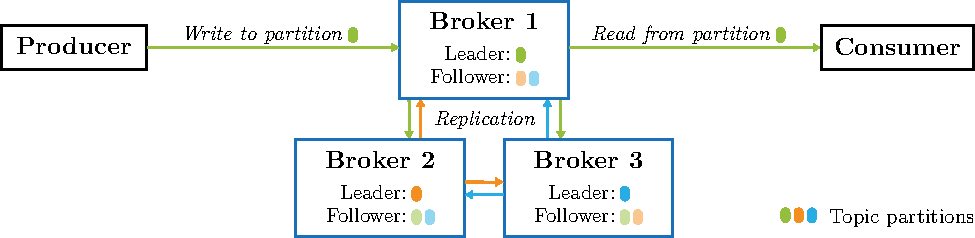
\includegraphics[width=\textwidth]{platforms_kafka_cluster}
	\caption[Structure of a Kafka cluster]{Structure of a Kafka cluster: partitions of a topic are spread across brokers acting as leader and follower replicas}
	\label{fig:platforms-kafka-cluster}
\end{figure}

Kafka supports flexible consumption patterns as previously shown in figure~\ref{fig:background-multiconsumer-patterns} using \emph{\glspl{consumer group}}. Each partition of a topic is assigned to one consumer in a consumer group. Therefore, load balancing can be achieved when every consumer belongs to the same consumer group. On the other hand, if all consumers are part of different consumer groups, every consumer receives all records for fan-out. Mixed patterns are also possible by having multiple consumer groups with multiple consumers. When using the load balancing pattern, Kafka effectively acts like a traditional message queue, whereas fan-out is more similar to publish--subscribe semantics. Offsets between consumers of a consumer group are coordinated via special topics, which becomes necessary when consumers within a group change and partitions need to be rebalanced between consumers. Consumers commit their offsets regularly to avoid duplicate consumption.

An important design decision is the use of consumer polling instead of broker pushing of records. This allows consumers to control the pace of consumption and not be overwhelmed, but also enables simple seeking to read from an earlier or later offset. Kafka brokers use a zero-copy method when serving consumers, which means that Kafka sends records directly from disk to network without intermediate buffers, which is enabled by using the wire format for storage. Multiple brokers called \emph{\glspl{bootstrap server}} can be specified in the consumer for the initial connection to the cluster, after which the consumer can ask for the desired partition leader.

Producers also use bootstrap servers to connect to the partition leader for appending records to the log. Producers can control how many replicas must have received the record before the write can be considered successful. With zero-acknowledgement, a producer may not wait for a reply from the partition leader at all to achieve very high throughput. With single-acknowledgement, a producer may wait for a success reply from the leader to be able to retry in case of leader failure. At the highest level of write safety but also the highest latency, a producer may wait for all in-sync replicas to have received and acknowledged the message. Producers can also batch multiple records into one write request to improve throughput at the cost of latency. Events must be serialized before being stored as binary payload in a record. Kafka provides basic serializers, but often custom serializers based on JSON or a generic serialization library like Avro\footnote{\url{https://avro.apache.org/}}, Protocol Buffers\footnote{\url{https://developers.google.com/protocol-buffers}} or Thrift\footnote{\url{https://thrift.apache.org/}} is used. Kafka also supports transactions for atomic writes of multiple records across multiple partitions, which enables producers to implement exactly-once stream sinks. To prevent the consumption of records of uncommitted transactions, consumers must support the isolation level directive.

The partition a new record will be assigned to is determined by a partitioner. The default partitioner assigns partitions based on a key like a user identifier or at random if none is given, but custom partitioning strategies are supported. Random partitioning balances partitions evenly while key-based partitioning might lead to high imbalances with hot keys. Depending on the configuration, records sent from a single producer may or may not be appended to the partition in the same order in case of retries.

Due to Kafka's popularity, a rich ecosystem of commercial offerings and libraries has emerged. Confluent, a company founded by one of the inventors of Kafka, provides a commercial Kafka platform with features like schema registries (centralized store for serialization schemas to be shared between consumers and producers) and tiered storage (offloading of old retained data from broker nodes to cheaper and scalable store like S3, also accelerating failure recovery and cluster rebalancing). Cloud platform providers like Amazon and Google also have fully managed offerings for Kafka, combining the flexibility and configurability of Kafka with the ease of operation of Kinesis Data Streams. Other tools like Kafka Connect allow the ingestion of streams from other systems to integrate Kafka into existing technology landscapes, and even more tools exist to mirror whole clusters, monitor performance and availability or run queries on streams.





\section{Stream Processing Platforms}
Stream processing platforms are also part of the stream transport platform ecosystem, consuming and producing streams while doing processing in between. They can also act as bridge between different transport platforms. The platform facilitates the development of processing jobs by taking care of aspects like event-time ordering, fault tolerance of state and scalability, and providing APIs to perform transformations on streams like windowing or pattern recognition. There is a number of frameworks with different approaches and paradigms that have been tried over time, refer to \cite{Fragkoulis.2020} for a comprehensive overview of the evolution and features of stream processing systems. We will focus on modern frameworks that can guarantee correct and consistent results through exactly-once processing. Therefore, we will not regard Samza\footnote{\url{http://samza.apache.org/}} (which only supports at-least-once processing), Spark Streaming (which has no support for event-time ordering and uses micro-batching) and Storm (although rudimentary stateful processing is supported with the Trident extension). However, they might still be suitable for certain applications. For example, Spark Streaming can leverage the extensive machine learning features of the Spark ecosystem. Kafka Streams\footnote{\url{https://kafka.apache.org/documentation/streams/}}, Spark Structured Streaming\footnote{\url{https://spark.apache.org/docs/latest/structured-streaming-programming-guide.html}}, Hazelcast Jet\footnote{\url{https://jet-start.sh/}} and Flink are open-source stream processing frameworks which are suitable for general stream analytics. All frameworks support high throughput and low latency, but exact numbers depend on the workload and configuration and will therefore not be compared here. Some performance results are presented in~\cite{Shahverdi.2019}. Note that all frameworks are under active development and new features are developed constantly, therefore existing limitations might be overcome.

Kafka Streams is a lightweight processing framework designed to run alongside the transport cluster, simplifying deployment because no separate cluster is needed but limiting it to Kafka as stream transport platform. Low-latency exactly-once processing with event-time ordering is supported. State can be queried from external applications and is stored in special compacted changelog topics for fault tolerance. Kafka Streams also transparently handles rebalancing of partitions when adding and removing processing instances through consumer groups. Kafka Streams applications perform stateless or stateful transformations on stream and table abstractions as well as joining and windowing. While not having the flexibility of the Dataflow mode, windowing in Kafka streams supports all three common window types and early/late triggers. In general, Kafka Streams is suitable for many processing types but is limited to Kafka sources and sinks, and the simple deployment lacks the flexibility of a dedicated cluster.

Spark Structured Streaming is a stream processing API built on top of the Spark batch processing framework. Jobs can be submitted to regular Spark clusters and run there in a scalable and fault-tolerant fashion. Kafka and Kinesis Data Streams can be used as stream sources and sinks. Jobs can be run in two modes. Exactly-once processing can be guaranteeed in micro-batching mode, while only at-least-once processing is possible in continuous processing mode. However, latencies can only be as low as \SI{100}{\milli\second} in micro-batching mode whereas latencies of \SI{1}{\milli\second} can be achieved with continuous processing. Spark Structured Streaming supports all common stream operations, but uses the latest event timestamp as watermark, which can lead to incorrectly discarded data in case of varying event-time skew~\cite[p.~386]{Akidau.2018}. Spark Structured Streaming does not use a dataflow graph processing model but uses an incremental version of the static queries on an unbounded table from the batch API~\cite[p.~601]{Armbrust.2018}. Compared to other frameworks, Spark Structured Streaming has not many unique advantages. However, stream processing jobs can be run on an existing Spark cluster and existing developer know-how from Spark batch jobs can be applied to Spark Structured Streaming.

Hazelcast Jet is the the newest of the four frameworks, having been released in 2018 with focus on high performance and easy maintenance~\cite{Hazelcast.2017}. Hazelcast Jet is built on top of the Hazelcast In-Memory Data Grid to support distributed in-memory data structures and lookups for stream enrichment. Jobs can be run on a a cluster for scalability and fault tolerance. The framework comes with many connectors for sources and sinks, and supports exactly-once processing with Kafka. While it has no SQL-like API, common stream operations with event-time ordering are supported, including early triggers. It also integrates with change data capture software for relational databases and supports batch processing with a similar API to stream processing. Coroutines with shared threads instead of individual threads are used for executing tasks, maximizing CPU utilization and reducing context switching overhead. Hazelcast Jet is a promising stream processing engine, but still immature due to its young age.

While Beam\footnote{\url{https://beam.apache.org/}} is not a stream processing engine, it is still worth mentioning in this context. Beam is an abstraction layer that allows to write stream and batch processing jobs which can be executed on a number of stream execution frameworks, including Flink, Hazelcast Jet, Spark and Samza but also Google's fully managed Cloud Dataflow\footnote{\url{https://cloud.google.com/dataflow/}} platform. Beam is one implementation of the Dataflow paper~\cite{TylerAkidau.2015} and therefore provides an API for all windowing concepts presented earlier. While Beam was designed as portability layer for jobs, the exact features like exactly-once processing and window output modes are dependent on the underlying stream execution framework.



\subsection{Apache Flink}
Flink is one of the most popular and powerful distributed processing framework~\cite[p.~54]{Shahverdi.2019} for stream and batch jobs. It was the first open-source platform to support event-time ordering and guarantee exactly-once processing with consistent managed state while achieving high throughput and low latency~\cite[p.~37]{Carbone.2015}. Flink is successfully being used in production for search index building, online machine learning, real-time activity monitoring and alerting, dynamic ride pricing and continuous ETL~\cite{Apache.2020c}. There also is a number of fully managed and commercial offerings for Flink. The framework can connect to a number of sources and sinks, including Kafka, Kinesis Data Streams, RabbitMQ, ActiveMQ, Cassandra, Redis and HDFS. Refer to \cites{Carbone.2015}{Friedman.2016} and the official documentation for more detailed information on job development for Flink as well as its internals.

The Flink stack is shown in figure~\ref{fig:platforms-flink-stack}. Flink can run on a single node during development, but is usually distributed across nodes as a cluster, possibly on top of a resource manager like YARN or Mesos, or containerized on Kubernetes. The runtime which executes dataflow graphs sits at the core of Flink. Dataflow graphs are specified using the DataSet API for batch processing or DataStream API for stream processing. Using the same engine for both bounded and unbounded data is possible since batch datasets are effectively special streams that are complete at the time of processing. However, the dataflow graphs and their execution on the runtime are optimized for either type. For example, operators in the graph are blocking when processing bounded datasets. This means that the entire dataset is processed by the operator before forwarding the intermediate stream to the next operator. This stages scheduling increases latency but is more efficient than continuous processing which is necessary for streams. On top of these two APIs, Flink comes with domain-specific libraries for graph processing and pattern recognition, with a machine learning library being under active development. Additionally, operations known from relational databases on streams and bounded datasets are possible using the table API or SQL. These levels of abstraction allow job developers to trade off between conciseness and expressiveness of the programming model, and open up stream processing to more users, possibly even non-experts who are only familiar with SQL.

\begin{figure}
	\centering
	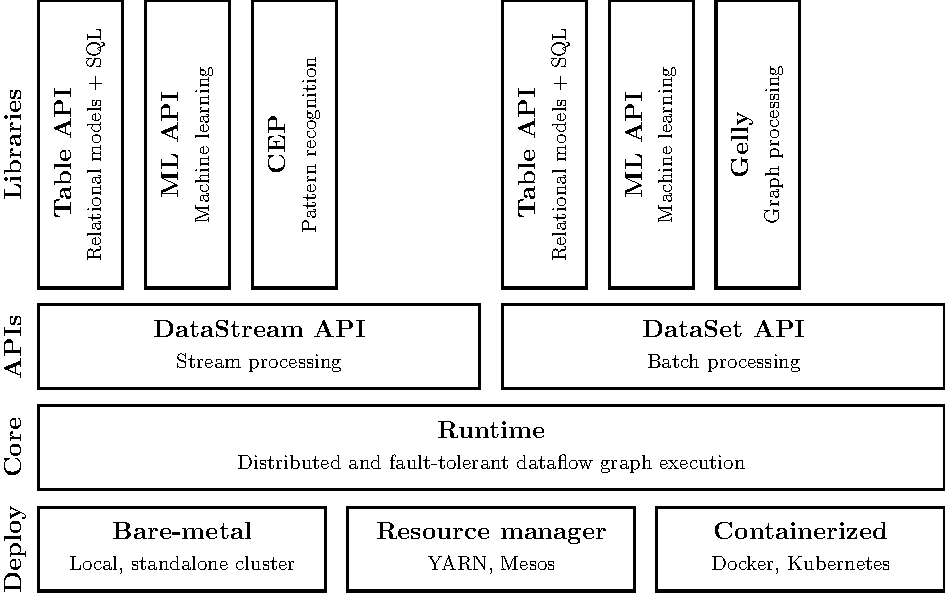
\includegraphics[width=\textwidth]{platforms_flink_stack}
	\caption[Components of Flink stack]{Components of Flink stack: multiple layers of abstraction run on top of diverse deployment environments}
	\label{fig:platforms-flink-stack}
\end{figure}


\subsubsection{API and Time Handling}
We will focus on operations on streams using the DataStream API. Common stream operations like \texttt{filter} and \texttt{map} but also splitting of a stream into multiple streams as well as joining of records of multiple streams based on some key are supported. Streams can be logically partitioned into keyed streams using the \texttt{keyBy} operation based on a key selector. All supported operators can be found in~\cite{Apache.2020d}. Arbitrary operations are possible using low-level process functions, which have access to stream records, can store fault-tolerant state, and can set timers in processing time and event time. This allows to implement transformations for which built-in operators do not offer enough control. Streams can also be enriched with external data using asynchronous functions to make database requests, query external APIs, run machine learning inference or execute other operations that may take long. Asynchronous functions handle timeouts and stream ordering while keeping latency low.

Windowing is a common operation to divide the unbounded stream into bounded datasets. Flink's windowing is inspired by the Dataflow model. Records are assigned to windows using a window assigner. Out of the box, tumbling, sliding and session windows are supported, but implementing custom window assigners is possible. Every window is aligned with epoch by default, which means that, for example, hourly windows start on the hour. Records emitted from a window carry the window end timestamp, which allows windows to be chained. This choice of timestamp also means that the delay introduced by chained windows is not additive. For example, chaining a \SI{15}{\minute} and a \SI{30}{\minute} introduces only \SI{30}{\minute} instead of \SI{45}{\minute} of latency. Flink provides two types of transformations on the records of a window. Reducing and folding transformations like summing or averaging aggregate records eagerly, which reduces state size, especially for large windows. Arbitrary transformations are supported using process window functions, but require Flink to buffer all records for a window. Since a copy of each record is created for every window it belongs to, this can quickly lead to large states. For example, there will be 86,400 copies of every record when using a sliding window of 1 day and an evaluation period of 1 second without eager aggregation. Flink supports completeness triggers, but only count-based triggers are supported for repeated updates. Custom triggers are supported to implement custom early/on-time/late triggers for balancing latency and correctness. Flink supports the delta and value output modes, but retractions must be implemented manually. Window evictors are not part of the Dataflow windowing model, but provide a way to remove certain records from the window before and after evaluation, which can for example be used for deduplication. However, the use of evictors prevents eager aggregation.

Processing data in the right time domain is crucial for correct results. Flink supports ordering of records by event time and processing time. The event timestamp can be extracted from records using a timestamp assigner, which also allows to use the ingestion timestamp (the time at which a record enters the Flink cluster) as event timestamp. Watermarks can be generated based on the event timestamps and emitted periodically (every \SI{200}{\milli\second} by default) or punctuatedly (when special records are observed). Flink ships with two periodic watermark generators. Watermarking for monotonously increasing timestamps assumes that records arrive in order with increasing timestamps, therefore the watermark follows the latest event timestamp. Watermarking with bounded out-of-orderness makes the watermark lag a fixed amount of event time behind the latest event timestamp. It is not recommended to emit watermarks at a very high frequency or even for every record, since watermarks usually trigger downstream computations which would degrade performance. The default period of \SI{200}{\milli\second} is suitable for most applications.

Watermarks originate at sources in the dataflow graph, and are then propagated downstream. Simple operations like \texttt{map} simply forward watermark, while more complex operators like windows only forward watermarks after emitting the results of the window computation. Therefore, windowing adds to the latency of the watermark like it does to regular records. Join operators, which have multiple inputs, use the minimum of all incoming watermarks.


\subsubsection{Architecture and Execution Model}
A Flink cluster comprises a client, a \emph{\gls{job manager}} and one or more \emph{\glspl{task manager}}, as shown in figure~\ref{fig:platforms-flink-cluster}. In most production cases, a separate \emph{\gls{per-job cluster}} for each job is recommended for resource isolation and limited impact of failures. However, shared \emph{\gls{session cluster}} are also possible for better resource utilization. The client creates and optimized a dataflow graph from the job specification and submits it to the job manager. The job manager coordinates the distributed execution of the dataflow on the task managers. This includes tracking the state and progress of each operator and intermediate stream between operators, but also coordinating checkpoints and recovery. While there is only one active job manager at any given time, failover is supported by promoting a standby job manager using a Zookeeper-based election. This eliminates the job manager as single point of failure for high availability. Task managers are JVM processes that execute operators and report their status to the job manager. Every task manager offers a certain number of \emph{\glspl{task slot}} (usually equal to the number of CPU cores) which determines how many tasks can be run in parallel by the task manager. Equal portions of the task manager's memory are allocated for each task slot. Inter-task manager communication to exchange intermediate streams is handled through direct network connections, which contain mechanisms for flow control to propagate backpressure from operators to sources. The network stack is detailed in~\cite{Apache.2019} with considerations for trading off latency and throughput. Any object needs to be serialized before transfer. Flink uses type inference to find the appropriate serializer/deserializer for a specific object, and provides optimized implementations for different data types. Custom serializers can be provided in for unsupported types.

\begin{figure}
	\centering
	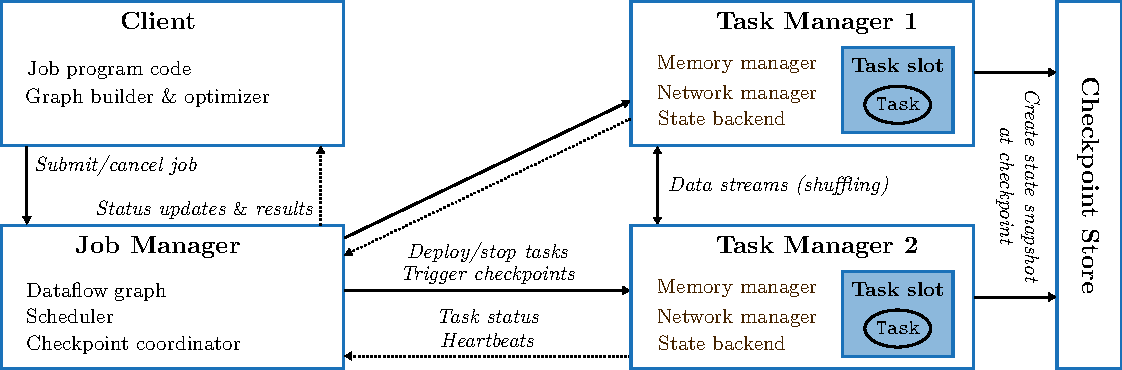
\includegraphics[width=\textwidth]{platforms_flink_cluster}
	\caption[Cluster architecture of Flink]{Cluster architecture of Flink: jobs running on task managers are coordinated by a job manager}
	\label{fig:platforms-flink-cluster}
\end{figure}

While the dataflow graph shows the logical structure of the job, it is parallelized for physical execution. This is shown in figure~\ref{fig:platforms-flink-dataflow}. Operators are split into one or more parallel instances called \emph{\gls{subtask}}, and streams are split into one or more partitions. The degree of parallelism can be defined for each operator. Parallelization results in two types of inter-subtask stream distribution patterns. Redistribution is necessary in case two subsequent operators do not have the same number of subtask, or when streams need to be shuffled after a \texttt{keyBy} operation. \emph{\Gls{network shuffling}} denotes the routing of records to a different task slot (possibly on a different node) since records with the same key need to be processed by the same subtask. Subsequent operators with the same number of subtasks and without shuffling result in one-to-one streams which preserves stream partitioning. Each subtask usually runs in its own thread. Some subsequent subtasks can also be chained to run in the same thread, which reduces the overhead of inter-thread buffering to improve throughput and latency. A \emph{\gls{task}} comprises either a subtask chain or an individual unchained subtask. Multiple successive tasks are allowed to occupy the same task slot through slot sharing, which enables running one parallel instance of the whole pipeline in one task slot. This yields better resource utilization and limits the number of required task slots to the maximum degree of parallism of a job instead of additionally being dependent on the number of operators.

\begin{figure}
	\begin{subfigure}[c]{\textwidth}
		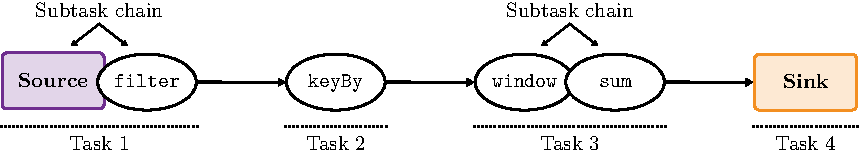
\includegraphics[width=\textwidth]{platforms_flink_dataflow_condensed}%
		\subcaption{Logical view}
		\label{fig:platforms-flink-dataflow-condensed}
	\end{subfigure}
	
	\bigskip

	\begin{subfigure}[c]{\textwidth}
		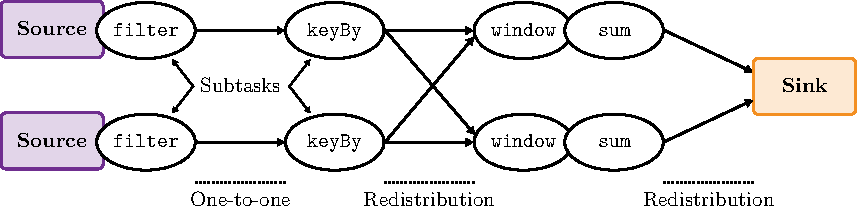
\includegraphics[width=\textwidth]{platforms_flink_dataflow_parallel}%
		\subcaption{Parallel view}
		\label{fig:platforms-flink-dataflow-parallel}
	\end{subfigure}
	\caption[Logical and parallel view of dataflow graph]{Logical and parallel view of dataflow graph: subtasks are parallel operator instances with one-to-one or redistribution partitioning patterns in between. Each parallel pipeline of tasks can occupy the same task slot, with each subtask (chain) running in a separate thread.}
	\label{fig:platforms-flink-dataflow}
\end{figure}

\subsubsection{State and Checkpointing}
Many operations like windowing and pattern recognition require state. Instead of storing the state in memory, state can be stored in the cluster so it can participate in checkpointing for fault tolerance. Flink provides interfaces to declare value, list and map states with optional time-to-live. State in operators can either be scoped to a key or a whole subtask. A special state type is broadcast state, which is available to all subtasks and is often used to update rules for alerting or parameters for machine learning. State can also be queried from the outside. Flink supports three state backends, which determine where state is stored. The memory state backend stores state in the job manager's memory and is only recommended during development. The file system and RocksDB backends write state to disk. Since this state is stored locally and maintained in memory as well if possible, performance is usually not impacted much. RocksDB allows keeping very large state and is recommended for production.

State can be regularly \glslink{checkpointing}{checkpointed} for fault tolerance by taking a state snapshot (possibly incremental in case of RocksDB) and storing it to a durable medium like HDFS or S3 known as snapshot store. Flink uses barriers inserted into the regular stream to notify operators of checkpointing and dividing the stream into a part which will be included in the current snapshot and a part which will be snapshotted later. An efficient algorithm is used to align barriers in case of \texttt{join} operators with multiple input streams. Snapshots also include input offsets of sources like Kafka and scheduled timers to guarantee end-to-end exactly-once processing even after failure recovery. The mechanism is detailed in ~\cite{Carbone.2017}. \emph{\Glspl{savepoint}} are a special kind of manually triggered checkpoint that can be used to stop and resume Flink jobs to perform code updates or maintenance, rescale by changing the parallelism, or fork the job for A/B testing or red/blue deployment.

Flink provides a comprehensive set of features for correct, fault-tolerant, low-latency and scalable stream and batch processing. In combination with a distributed and durable log transport platform like Kafka, exactly-once processing and backpressure handling are guaranteed even at large scales. Together with the powerful DataStream and DataSet APIs, this makes Flink and Kafka suitable for a wide range of use cases.
